\begin{exercise}
    Consider the problem $-u''(x) = x^2$ on the unit interval with $u(0) = u(1) = 0$.
    Let $u = \sum_{k = 1}^N u_k \sin{(\pi k x)}$ and $v = \sin{(\pi l x)}$ for $l = 1, \ldots, N$, for e.g.\ $N = 10, 20, 40$ and solve $(1.9)$.
    What is the error in $L_2$ and $L_\infty$.
\end{exercise}

\begin{solution}
    In this exercise, we use the Galerkin method to solve the problem, wishing to solve the problem as $Au = b$, where
    \begin{align*}
        A_{ij} &= \int_\Omega k \nabla N_j \cdot \nabla N_i \, dx, \\
        b_i &= \int_\Omega f N_i \, dx + \int_{\partial \Omega_N} h N_i \, ds.
    \end{align*}
    We begin by noting that
    \begin{equation*}
        \nabla N_i = \frac{d}{dx} \sin{(\pi i x)} = \pi i \cos{(\pi i x)},
    \end{equation*}
    such that
    \begin{align*}
        \int_\Omega k \nabla N_j \cdot \nabla N_i \, dx
        = \int_0^1 k \pi^2 i j \cos{(\pi j x)} \cos{(\pi i x)} \, dx
        = \frac{\pi^2 i^2}{2} \delta_{ij}.
    \end{align*}

    As we are given that the Dirichelt boundary conditions cover the entire boundary, and $\partial \Omega_D \cap \partial \Omega_N = \emptyset$, we have that the Neumann boundary integral is zero.
    The $b$ vector is then given by
    \begin{align*}
        b_i &= \int_\Omega f N_i \, dx
        = \int_0^1 x^2 \sin{(\pi i x)} \, dx
        = \frac{(2 - \pi^2 i^2)(-1)^i- 2}{\pi^3 i^3}.
    \end{align*}

    Setting up and solving the system for varying $N$ is then rather simples, implemented in \verb|exercise_1_1.py|.
    This gives the errors presented in Table~\ref{tab:1_1}, with the plotted solution in Figure~\ref{fig:1_1_curve}.
    \begin{table}[!h]
        \caption{Errors of approximations of $u$ for varying $N$, with sine basis functions.\label{tab:1_1}}
        \centering
        \begin{tabular}{lrr}
            \toprule
            $N$ & $L_2$ & $L_\infty$ \\
            \midrule
            10 & 0.001791 & 0.000224 \\
            20 & 0.000338 & 0.000059 \\
            40 & 0.000062 & 0.000015 \\
            \bottomrule
        \end{tabular}
    \end{table}

    \begin{figure}[!h]
        \centering
        \begin{subfigure}[b]{0.45\textwidth}
            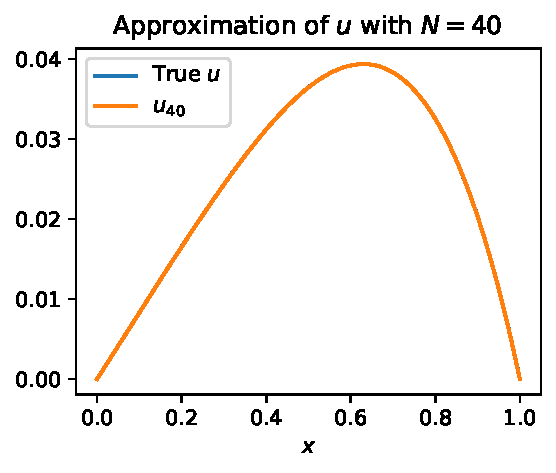
\includegraphics[width=\textwidth]{../figs/exercise_1_1.pdf}
            \caption{Approximated function.\label{fig:1_1_curve}}
        \end{subfigure}
        \hfill
        \begin{subfigure}[b]{0.45\textwidth}
            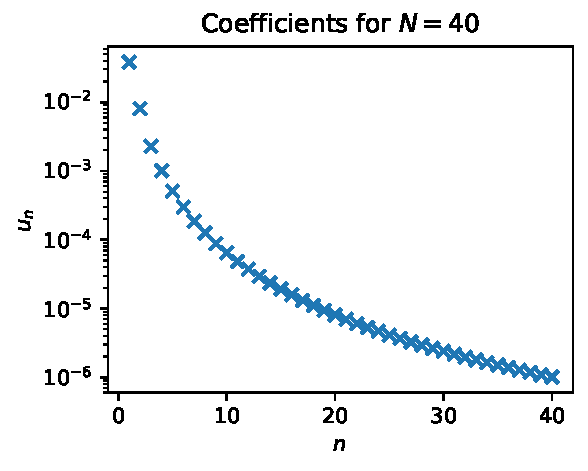
\includegraphics[width=\textwidth]{../figs/exercise_1_1_coeffs.pdf}
            \caption{Coefficients $|u_k|$.\label{fig:1_1_coeffs}}
        \end{subfigure}
        % 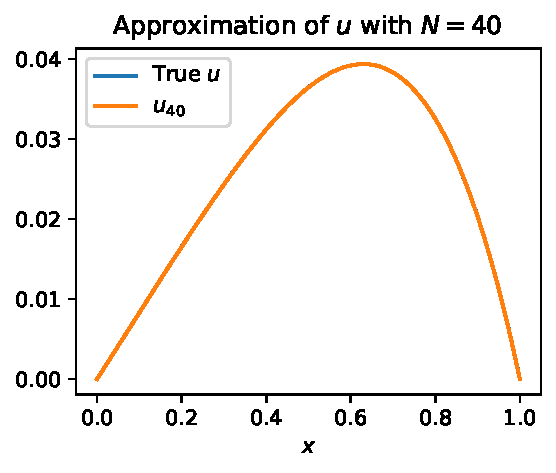
\includegraphics[width=0.7\textwidth]{../figs/exercise_1_1.pdf}
        \caption{Approximation of $u$ with $N = 40$ sine basis functions.\label{fig:1_1}}
    \end{figure}
\end{solution}
